\section{Introduction}
%-------------------------------------------------------------------------------
\label{sec:intro}
% With the widespread use of social networking services and other internet services, 
% Graph analytics is a useful tool to extract valuable statistics or 
Graph statistics is a useful tool for finding the structure or meaningful patterns in various graph data; e.g., social networks, e-mail networks, co-actor networks, and citation networks. 
For example, 
% when each node represents an individual, 
a \textit{degree} (i.e., number of edges connected to a node) in a social graph represents the number of friends for a single user, and a degree distribution represents a distribution of the number of friends over the whole graph. 
% Counting \textit{subgraphs} (e.g., triangles, stars, cliques) a fundamental task of analyzing 
\textit{Subgraph counts} 
(e.g., the number of triangles, stars, or cliques) provide fundamental information about the connection patterns in a graph (recent surveys can be found in \cite{Ribeiro_arXiv19}). 
The \textit{clustering coefficient}, which is the number of closed triplets (tuples consisting of three nodes connected by three edges)
% ($=3 \times$ \#triangles) 
over the total number of 
triplets (tuples consisting three nodes connected by two or three edges), 
% closed triplets and open triplets (three nodes connected by two edges)
measures the average probability that a friend's friend is also a friend in a social network. 

While such graph statistics is important to understand the property of graphs, 
graph analysis often raises a serious privacy concern. 
% the graphs often involve sensitive data; e.g., some users may not want to reveal her friend list to strangers. 
For example, 
% a graph may involve 
edges could correspond to sensitive friendships 
% or sexual relationships 
that a user wants to keep secret. 
User attributes (e.g.,  gender, profession, dormitory) might also be inferred from a social network \cite{Dougnon_AI15,Mislove_WSDM10}.
Therefore, it is desirable to develop an algorithm for analyzing graph statistics while protecting user privacy.

% Privacy-preserving graph analysis 
Differentially private analysis of graphs \cite{Raskhodnikova_Encyclopedia16} has been widely studied to release graph statistics while providing DP (Differential Privacy) \cite{DP,Dwork_ICALP06}. 
DP protects user privacy against adversaries with arbitrary background knowledge, and is known as a gold standard for data privacy. 
A vast majority of DP on graphs assume the \textit{centralized (or global) model} \cite{blocki2012johnson,Chen_PoPETs20,Day_SIGMOD16,Hay_ICDM09,Karwa_PVLDB11,Kasiviswanathan_TCC13,Nissim_STOC07,Raskhodnikova_arXiv15,Raskhodnikova_Encyclopedia16,Song_arXiv18,Wang_PAKDD13,Wang_TDP13}, where a single trusted data curator holds the entire graph and releases sanitized versions of the graph statistics. 
By assuming a trusted party that can access the entire graph, 
% In this model, 
it is possible to release accurate graph statistics 
(e.g., subgraph counts \cite{Karwa_PVLDB11,Kasiviswanathan_TCC13,Song_arXiv18}, degree distribution \cite{Day_SIGMOD16,Hay_ICDM09,Raskhodnikova_arXiv15}, 
spectra 
% eigenvalues and eigenvectors 
\cite{Wang_PAKDD13}) 
or synthetic graphs \cite{Chen_PoPETs20,Wang_TDP13} 
while strongly protecting user privacy. 

However, 
it might be difficult to assume that a single trusted party can access the entire graph in practice. 
% the assumption of a single trusted data curator can be strong in practice. 
For example, the number of data breaches is increasing in recent years \cite{data_breach1,data_breach2}. 
Therefore, 
% it is not hard to imagine that 
the entire graph may be leaked from the data curator by illegal access or internal fraud. 
For another example, there is no centralized server in \textit{decentralized social networks} \cite{Paul_CN14,Salve_CSR18}; e.g., Diaspora \cite{Diaspora} uses many servers all over the world, each containing the data of users who have chosen to register it. 
% ; In Mastodon \cite{Mastodon}, a user can run her own server. 
In this case, there is no server that has the entire graph. 
Furthermore, we can also consider a fully decentralized application in which a server does not have any (original) edge between users. 
% i.e., local model. 
For example, suppose a mobile application that asks users how many of their friends they have seen today and sends its noisy version to a central server. 
In this application, the server does not hold any edge in the original graph, 
% (i.e., there is no trusted third party), 
but can still aggregate the responses to determine the average mobility in an area. 

The standard privacy metric when we do not assume any trusted third party is LDP (Local Differential Privacy) \cite{Duchi_FOCS13,Kasiviswanathan_FOCS08}. 
LDP is a special case of DP in the \textit{local model}, where each user obfuscates her personal data by herself and sends the obfuscated data to a (possibly malicious) data collector. 
Since the data collector does not hold the original personal data, it does not suffer from the data leakage issue explained above. 
Therefore, LDP has recently attracted attention from both the academic field \cite{Acharya_AISTATS19,Bassily_STOC15,Bassily_NIPS17,Fanti_PoPETs16,Kairouz_ICML16,Kairouz_JMLR16,Murakami_USENIX19,Qin_CCS16,Wang_USENIX17,Ye_ISIT17} and industry \cite{Erlingsson_CCS14,Ding_NIPS17,Thakurta_USPatent17}. 
% Most of the studies on LDP focus on 
However, LDP has mostly been used in the context of tabular data where each row corresponds to an individual, and little attention has been made on LDP for graph statistics (see 
Section~\ref{sec:related} for details). 
% Related work at the end of Section~\ref{sec:intro}). 

\begin{figure}
\centering
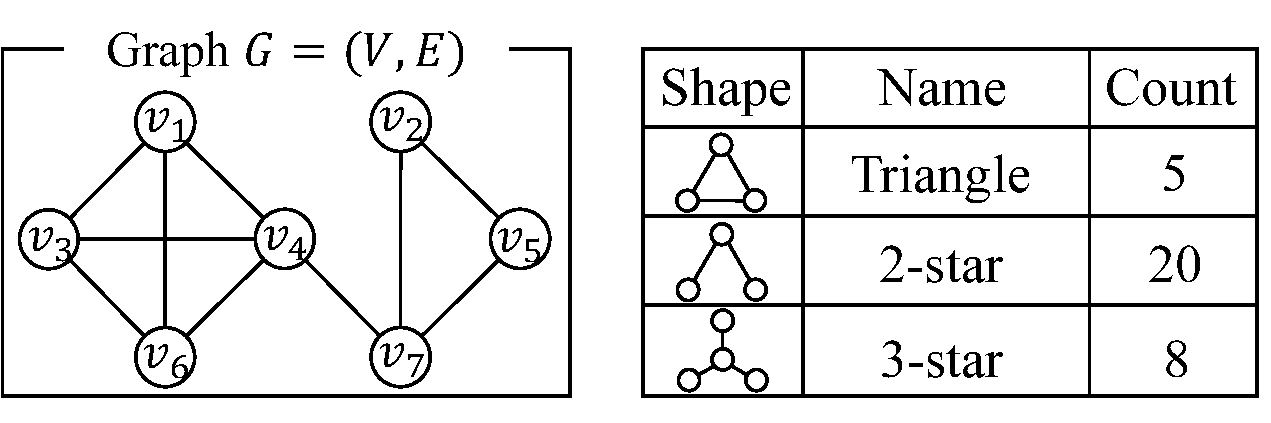
\includegraphics[width=0.9\linewidth]{fig/subgraph.pdf}
\vspace{-2mm}
\caption{Example of subgraph counts.}
\label{fig:subgraph}
\end{figure}

In this paper, we consider LDP for graph data, and 
% propose solutions 
provide algorithms and theory 
for calculating graph statistics in this model. 
In particular, we focus on counting triangles and $k$-stars, which are the most basic subgraphs. 
% such as triangles and $k$-stars. 
A triangle is a set of three nodes with three edges (we exclude automorphisms; i.e., \#closed triplets $= 3 \times$ \#triangles). 
A $k$-star consists of a central node connected to $k$ other nodes. 
Figure~\ref{fig:subgraph} shows an example of triangles and $k$-stars. 
Counting them is a fundamental task of analyzing the connection patterns in a graph. 
% , as explained above. 
% In addition, 
The clustering coefficient can also be calculated from triangle counts and $2$-star counts as: $\frac{3 \times \text{\#triangles}}{\#2\text{-stars}}$ (in Figure~\ref{fig:subgraph}, $\frac{3 \times 5}{20} = 0.75$). 

Counting subgraphs in the local model is very challenging. 
The main challenge is that existing LDP techniques and theory do not directly apply. 
The existing work on LDP for tabular data assumed that 
% each user's data value 
each data value to be counted 
is independently and identically distributed from an underlying distribution. 
% (see Section~\ref{sec:related}). 
In graphs, this is no longer the case; e.g., 
each triangle is not independent, because multiple triangles can involve the same edge; 
each $k$-star is not independent for the same reason. 
% both triangles and $k$-stars are not independent, because multiple triangles and multiple $k$-stars can involve the same edge. 
Moreover, complex interdependency involving multiple people is possible in graphs. 
For example, each user cannot count triangles involving her, because she cannot see edges between other users; 
e.g., in Figure~\ref{fig:subgraph}, user (node) $v_1$ cannot see an edge between $v_3$ and $v_4$. 

% This simultaneously presents both challenges and opportunities. 
Although the complex interdependency introduces challenges, it also presents opportunities -- the interdependency also implies that interaction between users and a data collector may be particularly helpful depending on the prior responses. 
In this work, we investigate this issue and provide algorithms for accurately calculating subgraph counts under LDP. 
% counts that use various levels of interaction. 

\smallskip
\noindent{\textbf{Our contributions.}}~~To our knowledge, this work is the first to 
% study the problem of 
provide algorithms and theory for 
counting triangles and $k$-stars in graphs under LDP. 
Our contributions are as follows:
\begin{itemize}
    \item For triangles, we first present an algorithm based on 
    Warner's RR (Randomized Response) \cite{Warner_JASA65} 
    and empirical estimation \cite{Kairouz_ICML16,Murakami_USENIX19,Wang_USENIX17}. 
    %and show that its estimation error is very large for a large number of users. 
    Then we present a more sophisticated algorithm using the interaction between users and a data collector. 
    %and show that it significantly reduces the estimation error.
    We analyze upper-bounds on the estimation error for both the algorithms, and show that the latter algorithm can  significantly reduce the estimation error. 
    \item For $k$-stars, we present a simple algorithm using the Laplacian mechanism. 
    %show that it accurately counts $k$-stars. 
    We analyze the upper-bound on the estimation error for this algorithm, and 
    %In particular, 
    show that 
    it is 
    %achieves 
    %the upper-bound on the estimation error of this algorithm is 
    order optimal 
    %estimation error 
    in terms of the number of users among all LDP mechanisms without interaction.
    \item We show lower-bounds on the estimation error for general functions including triangle counts and $k$-star counts. 
    The lower-bounds provide an insight into how accurate our algorithms are. 
    They also provide the limitations of the local model when compared to the centralized model.
    \item We evaluate our algorithms using two real datasets, and show that 
    it is indeed possible to accurately estimate 
    subgraph counts in the local model. 
    %Our experimental results show that 
    %although the algorithms in the local model provide high estimation errors than those in the centralized model,  
    In particular, we show that 
    the interactive algorithm for triangle counts and the Laplacian algorithm for the $k$-stars provide small estimation errors for a large number of users.
\end{itemize}

% \smallskip
% \noindent{\textbf{Related work.}}~~Here we explain the previous work related ours. 
